\section{Elementos de Configuración}\label{sec:elementosDeConfiguracion}

Nuestro proyecto de gestión de incidentes de búsqueda y rescate en el mar se compone de varios elementos de configuración que 
son fundamentales para su desarrollo y mantenimiento. Estos incluyen los productos de software, documentos y bases de datos, 
cada uno con sus propias características y procesos de gestión.

\subsection{Productos de Software}
El sistema se compone principalmente de dos aplicaciones: una aplicación web desarrollada en Next.js, que sirve como interfaz 
principal para los usuarios y gestora de los incidentes, y una API para integraciones con terceros como Sea Vision, NOAA e ITU.

\subsubsection{Control de cambios}
Para el control de cambios, utilizamos Git como sistema de control de versiones, alojando nuestro repositorio en GitLab. Esto nos 
permite rastrear todas las modificaciones realizadas en el código fuente, facilitando la colaboración entre los miembros del equipo 
y el mantenimiento de un historial detallado de los cambios.

\subsubsection{Estándares para el ramificado}
Hemos establecido un estándar de ramificación que nos ayuda a organizar el desarrollo de manera eficiente. Mantenemos dos ramas 
principales: \textit{main} y \textit{develop}. La rama \textit{develop} es nuestro ambiente de desarrollo principal, donde integramos todas las nuevas 
características y correcciones. Para nuevas funcionalidades, creamos ramas con el prefijo \textit{feature/}, para correcciones de errores 
usamos \textit{bugfix/}, y para soluciones urgentes en producción, \textit{hotfix/}. Este enfoque nos permite trabajar de forma paralela en diferentes 
aspectos del proyecto sin interferir con el trabajo de otros miembros del equipo.

[TODO: Incluir citas de flujo conocido. Opciones
- https://www.atlassian.com/git/tutorials/comparing-workflows/gitflow-workflow
- https://trunkbaseddevelopment.com/
- https://docs.github.com/en/get-started/using-github/github-flow
]

\subsection{Versionado}
Seguimos un esquema de versionado semántico (X.Y.Z) para nuestro proyecto. Las versiones 0.0.X se utilizan para cambios menores durante 
el desarrollo inicial. Las versiones 0.1.0 indican versiones de \textit{stage}, mientras que 0.1.X se usan para correcciones de errores o \textit{hotfixes} 
en \textit{stage}. Las versiones 1.0.0 y superiores se reservan para las versiones de producción. Este sistema nos permite comunicar claramente la 
naturaleza de los cambios en cada versión.

\subsection{Proceso de despliegue del servidor}
Nuestro proceso de despliegue varía según el ambiente. Para desarrollo, utilizamos un servidor on-premise que cuenta con Jenkins, SonarQube y Kubernetes. 
Cada push a la rama 'develop' desencadena un flujo de CI/CD que culmina con el despliegue automático en nuestro ambiente de desarrollo. Para el ambiente de 
producción del cliente, el proceso es manual: subimos el proyecto a su repositorio de código y actualizamos las versiones en su servidor de staging. 
Este servidor es on-premise, accesible vía VPN, y ejecuta el proyecto en contenedores Docker.

\subsubsubsection{Pipeline DevSecOps}
Contar con un ambiente de desarrollo bien estructurado y orientado a la estabilización del código es esencial para garantizar un flujo de trabajo eficiente, 
seguro y confiable. Este enfoque no solo mejora la calidad del producto final, sino que también facilita la colaboración entre los equipos de desarrollo, 
asegurando que el código esté siempre listo para ser desplegado a producción. A continuación, se destacan las razones clave:

\begin{enumerate}
    \item Código listo para despliegue\\
    Un ambiente de desarrollo estable asegura que el código pueda ser desplegado fácilmente en producción en cualquier momento. Esto implica que se 
    cumplen los estándares necesarios para evitar problemas al migrar funcionalidades desde el entorno de desarrollo hacia entornos de prueba o producción.
    \item Pruebas básicas de seguridad
    Incorporar pruebas de seguridad en el ambiente permite detectar vulnerabilidades comunes de manera temprana. Validaciones como el análisis estático de 
    código para detectar inyecciones, accesos no autorizados o datos expuestos son fundamentales para reducir riesgos en entornos de producción.
    \item Pruebas de calidad de código
    Un ambiente de desarrollo efectivo también incluye herramientas de análisis de calidad de código. Estas revisan aspectos como:
    \begin{itemize}
        \item Legibilidad y consistencia.
        \item Seguimiento de convenciones de codificación.
        \item Identificación de código duplicado o poco eficiente. Esto permite a los equipos mantener estándares altos, reducir la deuda técnica y facilitar 
        el mantenimiento futuro del software.
    \end{itemize}
    \item Pruebas automáticas de funcionalidades
    Las pruebas automatizadas garantizan que las funcionalidades implementadas cumplan con los requisitos establecidos. Estas pruebas permiten validar:
    \begin{itemize}
        \item El correcto funcionamiento de las nuevas características.
        \item La no alteración de funcionalidades existentes tras cambios en el código (regresión).
        \item La eficiencia y robustez del software bajo diferentes escenarios. Al integrar estas pruebas como parte del proceso, los equipos pueden detectar 
        errores rápidamente y corregirlos antes de que lleguen al usuario final.
    \end{itemize}
\end{enumerate}


\begin{figure}[H]
    \centering
    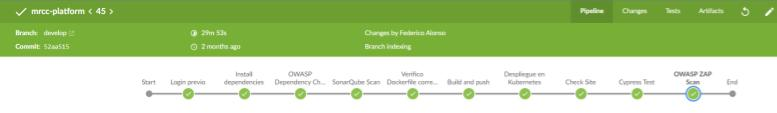
\includegraphics[width=0.8\textwidth]{../imagenes/secciones/7-Gestion-de-la-configuracion/Pipeline DevSecOps.jpg}
    \caption{Pipeline DevSecOps}
    \label{fig:devsecops}
\end{figure}

\begin{figure}[H]
    \centering
    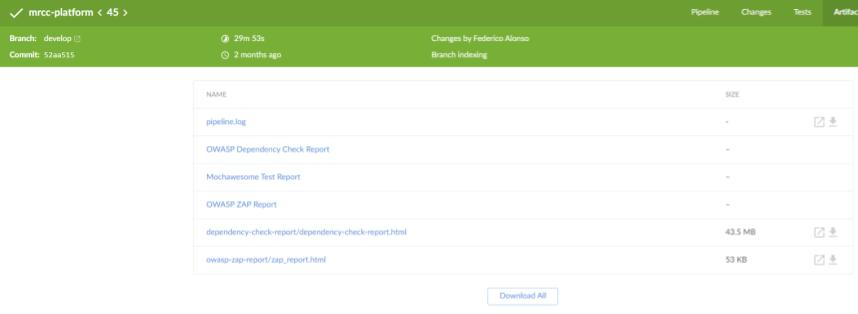
\includegraphics[width=0.8\textwidth]{../imagenes/secciones/7-Gestion-de-la-configuracion/ejecucion pipeline.jpg}
    \caption{Ejecución del pipeline}
    \label{fig:ejePipeline}
\end{figure}

\begin{figure}[H]
    \centering
    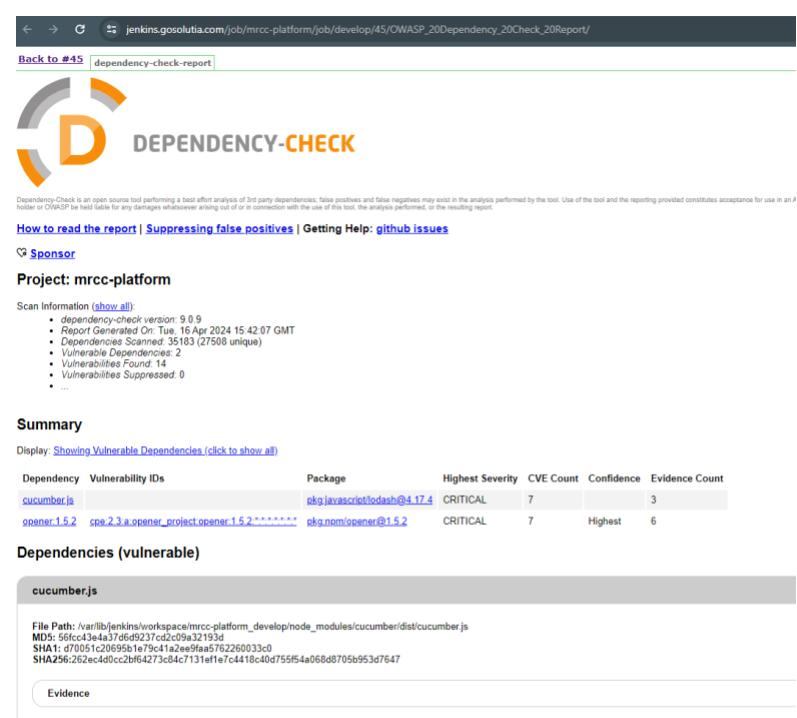
\includegraphics[width=0.8\textwidth]{../imagenes/secciones/7-Gestion-de-la-configuracion/OWASP - dependency check.jpg}
    \caption{OWASP - dependency check}
    \label{fig:owasp}
\end{figure}

\begin{figure}[H]
    \centering
    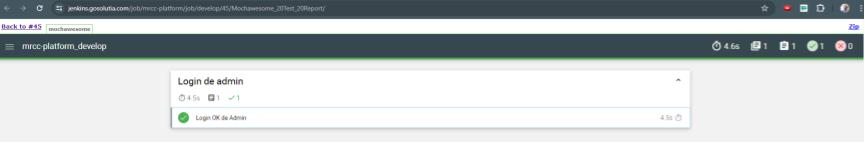
\includegraphics[width=0.8\textwidth]{../imagenes/secciones/7-Gestion-de-la-configuracion/Mochawsome report.jpg}
    \caption{Reporte Mochawsome}
    \label{fig:mochawsome}
\end{figure}


\begin{figure}[H]
    \centering
    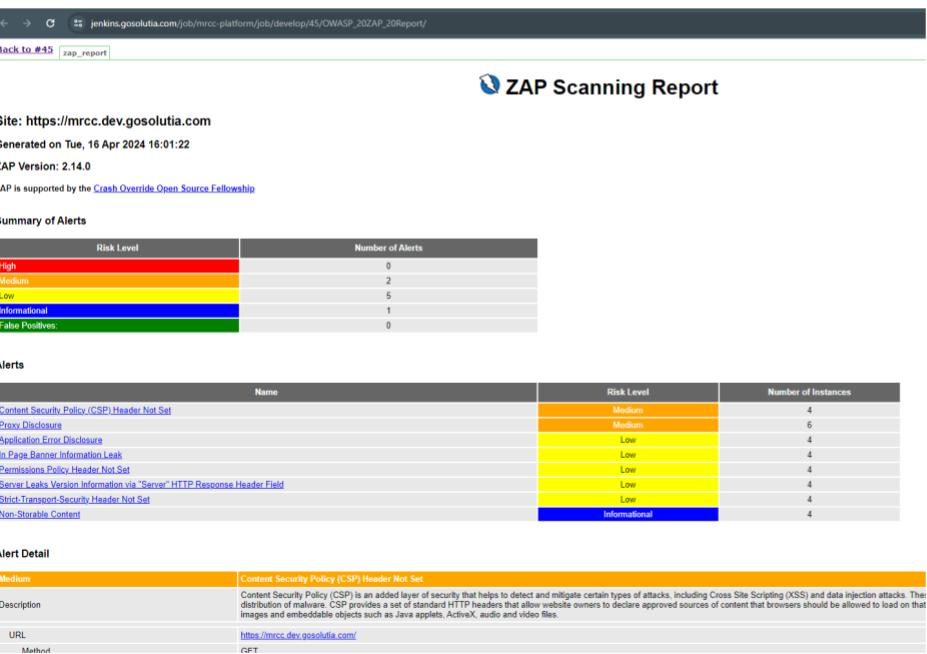
\includegraphics[width=0.8\textwidth]{../imagenes/secciones/7-Gestion-de-la-configuracion/ZAP Scan Report.jpg}
    \caption{Reporte de escaneo ZAP}
    \label{fig:zap}
\end{figure}

\begin{figure}[H]
    \centering
    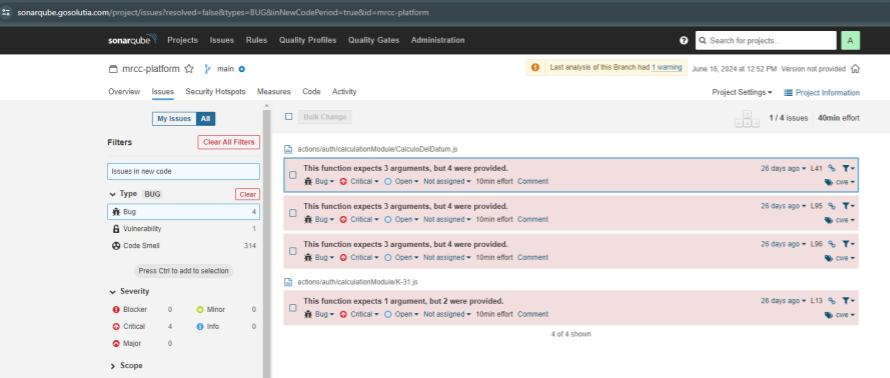
\includegraphics[width=0.8\textwidth]{../imagenes/secciones/7-Gestion-de-la-configuracion/SonaQube report.jpg}
    \caption{Reporte de SonarQube}
    \label{fig:sonarqube}
\end{figure}


\subsection{Documentos}
Gestionamos nuestra documentación principalmente a través de Google Drive. Este enfoque nos permite colaborar en tiempo 
real y mantener un registro actualizado de todos los aspectos del proyecto. Los documentos se van creando y actualizando 
a medida que avanzamos en las diferentes etapas del proyecto, asegurando que la documentación evolucione junto con el 
desarrollo del sistema.

\subsubsection{Bases de datos}
Para la gestión de bases de datos, utilizamos Prisma como ORM (Object-Relational Mapping). Esto nos proporciona una capa de 
abstracción que facilita las operaciones de base de datos y mantiene la consistencia en nuestro modelo de datos. Los scripts SQL 
para inserciones iniciales o configuraciones por defecto se almacenan en el directorio 'docs/sql' de nuestro repositorio en GitLab, 
lo que nos permite versionar estos cambios junto con el código de la aplicación.